\documentclass[a4paper, 12pt, titlepage]{article}
\usepackage[utf8]{inputenc}
\usepackage[T1]{fontenc}
\usepackage[magyar]{babel}
\usepackage{graphicx}

\begin{document}

\pagestyle{plain}
\part*{Általános Hook törvény, izotrop közegek rugalmas tulajdonságai} %Általános Hook törvény, izotrop közegek rugalmas tulajdonságai
\section*{Általános Hook törvény}
A továbbiakban vizsgáljuk a szilárd anyagok alakváltozásait! Ekkor ugye $\hat{\sigma}$ feszültségtenzor csak $\hat{\varepsilon}$ deformációstenzortól függ. Egysezrű nyújtás esetében megfigyelt jelenséget (azaz a folyáshatárig ($\sigma_{f}$) lineáris kapcsolatot -lásd \ref{fig:hook}.\hspace{1mm}ábra-) a lineáris Hooke-törvény írja le ($\sigma=E\varepsilon$).
	\begin{figure}[!h]
	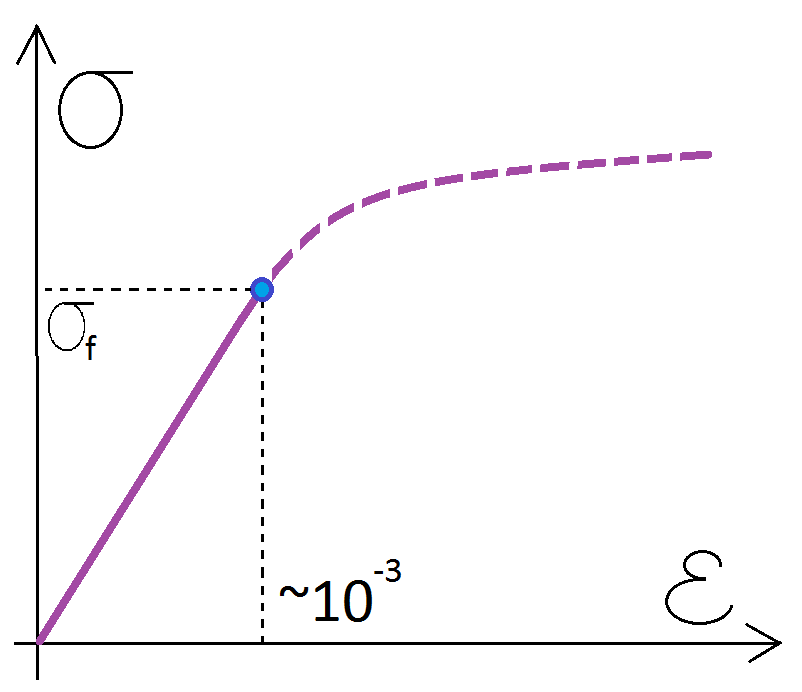
\includegraphics[height=3.5cm]{./hook.png}
	\centering
	\caption{Feszültség egyszerű nyújtás során deformáció függvényében (konstitúció).}
	\label{fig:hook}
	\end{figure}
$\underline{u}$-t, illetve $\hat{\varepsilon}$-t onnan mérjük, számoljuk, ahol a feszültség nulla; ez a referenciahelyzet.
\newline
Ezek alapján felírhatjuk az \textbf{általánosított Hooke-törvényt} indexesen: %hook
	\begin{equation}
\sigma_{ij}=c_{ijkl}\varepsilon_{kl}
	\label{eq:hook}
	\end{equation}
A lineáris kapcsolatot $c_{ijkl}$ teremti meg, ez a legáltalánosabb összefüggés, mely két tenzor közt lehet.
\newline
\Aref{eq:hook}.\hspace{1mm}egyenletet felírhatjuk mérnöki jelöléssel is, melynek lényege az indexek egybeejtésén alapszik. Ez történik ugyebár skaláris szorzás esetén is. Minthogy itt azonban tenzorokról van szó, a skaláris szorzásból ismert "$\cdot$"-t ":" váltja fel (mintha két skalásis szorzás lenne, s így két "$\cdot$" használatos). Illetve "c" két kalapot kap (1 kalap 2 index, 2 kalap $2\cdot 2=4$ index analógiájaképp). Ezzel a jelölésel élve \aref{eq:hook}.\hspace{1mm}egyenlet az alábbi alakot veszi fel:
\[\hat{\sigma}=\hat{\hat{c}}:\hat{\varepsilon}\]
\Aref{eq:hook}.\hspace{1mm}egyenletben szereplő $\hat{\hat{c}}$ azonban 81 konstanst jelentene (minden indexre hármat)... Ámde szerencsére tudjuk, hogy $\hat{\varepsilon}$ szimmetrikus, így ha $c_{ijkl}$ $kl$ indexekben nem lenne szimmetrikus, az úgyis kiesne $\hat{\varepsilon}$-nal való szorzáskor, tehát $c_{ijkl}$ $kl$ indexeiben szimmetrikus kell legyen. Ugyanezt elmondhatjuk $ij$ indexeiről is, mert $\hat{\sigma}$-ról is tudjuk, hogy szimmetrikus. Így ($6\cdot 6$) 36 független értékünk van. Ez azonban még mindig elkeserítően soknak tűnik.
\newline
Segítségünkre van a termodinamika gondolata, miszerint ha az atomok közt kizárólag konzervatív erők lépnek fel, akkor fel tudjuk írni az egész rendszer helyzeti energiáját. S ha a helyzeti energiát ismerjük az összes atom függvényében, akkor abból ki tudjuk számolni az $i$-edik atomra ható erőt úgy, hogy vesszük a potenciál negatív gradiensét. Ha viszont tudjuk, hogy az $i$-edik atomra milyen erő hat, akkor azt is tudjuk, hogy hogyan mozog. (Magyarán feltesszük, hogy az energiából mindenre tudunk következtetni, csak deriválni kell.) Ennek viszont igaznak kell maradnia a kontinuum-elmélet szintjén is. Próbáljuk hát kitalálni egy ilyen kontinuum rugalmas energiáját! %termo
\newline
Szemléletesen úgy is tekinthetünk a rugalmas testre, mintha benne az atomok rugókkal lennének összekötve. Így a köztük létrejövő kölcsönhatás konzervatív.
Vegyünk egy falhoz rögzített $l$ hosszú és $A$ keresztmetszetű rudat (vagy deszkát), melyet húzzunk $F$ erővel! Ennek hatására $\Delta x$-szel fog megnyúlni (\ref{fig:rud}.\hspace{1mm}ábra). 
	\begin{figure}[!h]
	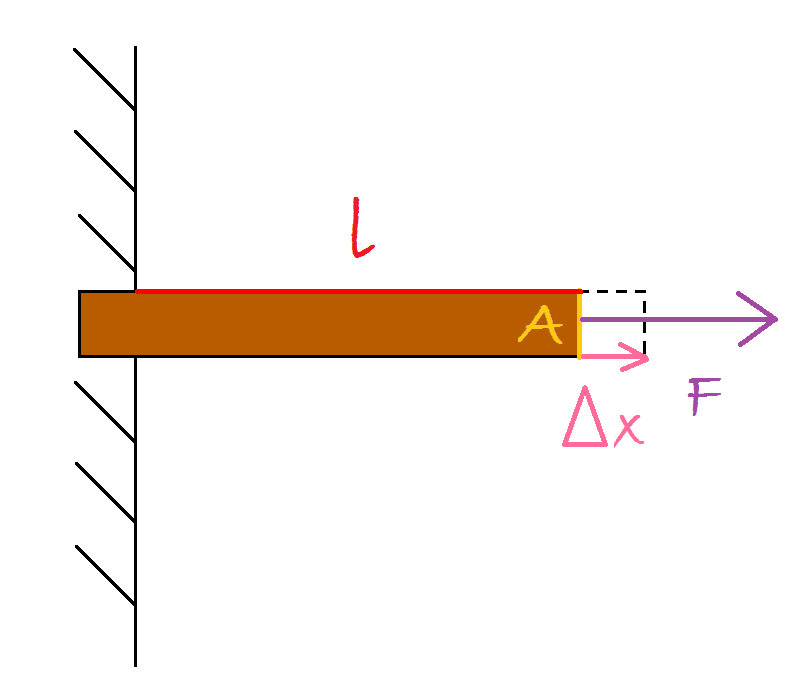
\includegraphics[height=3.5cm]{./rud.png} %rud.png
	\centering
	\caption{Rúd (/deszka) nyújtása.}
	\label{fig:rud}
	\end{figure}
Ekkor a végzett munka $W=\frac{1}{2}F\Delta x$ (Minthogy $\underline{F}$ és $\Delta\underline{x}$ vektorok közti $\varphi=0$, s így $\cos(\varphi)=1$, a két vektor skaláris szorzata megegyezik a vektorhosszak szorzatával.) Ám azt is tudjuk, hogy $F=\sigma A$, ahol $\sigma=E\frac{\Delta x}{l}$. Ha ezt osztjuk $V$-vel, és felhasználjuk, hogy $V=Al$; megkapjuk az egységnyi térfogatra jutó munkát a deformáció során, azaz $w$-t:
\[\frac{W}{V}=\frac{1}{2}E\frac{\Delta x}{l}\frac{\Delta x}{l}\]
egyszerűsítve
\[\frac{1}{2}E\varepsilon^{2}=w\]
Amely egyenlőséget több dimenzióra általánosítva megkapjuk az alábbi, $\hat{\varepsilon}$-ban kvadratikus alakot a \textbf{rugalmasenergia-sűrűségre}:
	\begin{equation}
w=\frac{1}{2}\varepsilon_{ij}c_{ijkl}\varepsilon_{kl} %w
	\label{eq:w}
	\end{equation}
Amiről pedig azt tudjuk mondani, hogy mivel jobbról-balról is $\hat{\varepsilon}$-nal szorzunk, $c_{ijkl}$ nem csak külön $ij$ és $kl$ indexeiben szimmetrikus, hanem első két indexét is megcserélhetjük a hátsó indexpárjával. Ennek pedig az lesz a következménye, hogy nem 36, csupán 21 független komponensünk van ($6\times 6$-os mátrix főátlóban levő, s afeletti -vagy alatti- komponensei: $1+2+3+4+5+6$ darab). Ennél még szebb a helyzet, ha az anyag kristályrács-szerkezete köbös, s így kocka-szimmetriája van, mivel a 21 úgy 3 független komponenssé redukálódik. Ilyenkor $90^{\circ}$-os forgatáskor az energia ugyanannyi; $\hat{\hat{c}}$ invariáns kell maradjon. S ugyan a kockarács (melyben a bázisvektorok páronként derékszöget zárnak be, s egyenlő hosszúak) erős megszorítást jelent, a fémek jelentős hányada tércentrált kockarácsban kristályosodik (például lítium, nátrium, kálium, bárium, króm, vas 1394-153$8^{\circ}$C közt -$1394^{\circ}$C alatt lapcentrált köbössé alakul, $1538^{\circ}$C-on pedig olvad-), de néhány ionrácsos anyag is (pédául a cézium-halogenidek -a CsF kivételével, mely lapcentrált köbös kristályrácsú-). %kristszerk
\newline
\Aref{eq:w}.\hspace{1mm}egyenletbe behelyettesítve $\hat{\sigma}$-t a Hooke-törvény (\ref{eq:hook}.\hspace{1mm}egyenlet) alapján indexesen:
	\begin{equation}
\sigma_{mn}=\frac{\mathrm{d}w}{\mathrm{d}\varepsilon_{mn}} %sigmatort
	\label{eq:sigmatort}
	\end{equation}
Ugyanis csak akkor nem nulla a kifejezés, ha $\varepsilon_{ij}$ és $\varepsilon_{kl}$ indexeit a szimmetriát felhasználva egybeejtjük ($\varepsilon_{mn}$).
\newline
\newline
\section*{Izotrop közegek rugalmas tulajdonságai}
Izotrop anyagnak nevezzük az olyan anyagokat, melyekben neincs kitüntetett irány. Azaz akárhogy (bármely irányból) vágunk is ki az anyagból kis darabkát, mindig ugyanúgy fog viselkedni (\ref{fig:izotrop}.\hspace{1mm}ábra). Ugyan például a kréta kisszemcsés (poli)kristályokból áll, makroszkopikusan tekinthető izotropnak (ellenben például egy majd méteres szilícium-egykristállyal).
	\begin{figure}[!h]
	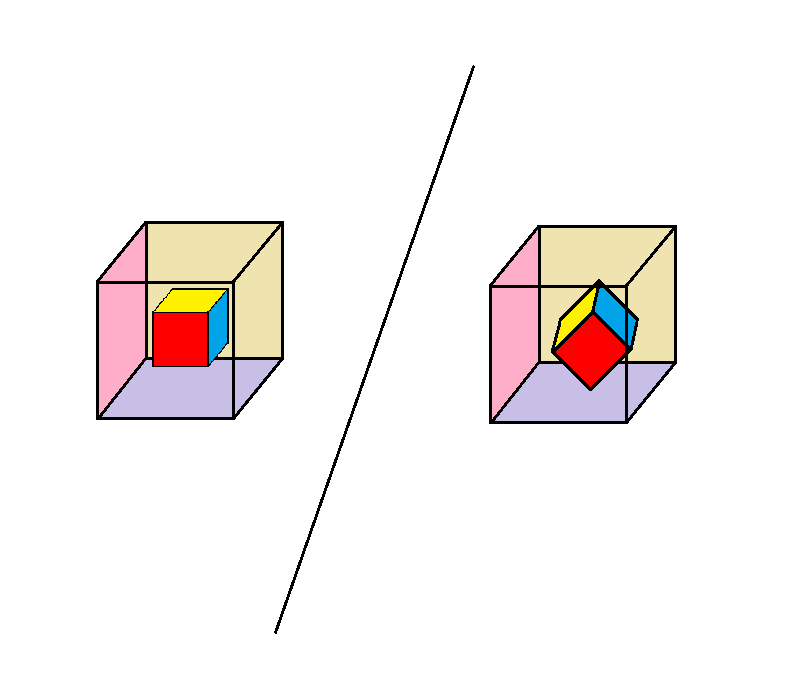
\includegraphics[height=3.5cm]{./izotrop.png} %izotrop.png
	\centering
	\caption{Különbözőképp kivágott anyagdarabok ugyanúgy viselkednek.}
	\label{fig:izotrop}
	\end{figure}
Az anyagok egy része kristályos szerkezetű, ezek jó közelítéssel izotropnak tekinthetők. Ilyen esetben $\hat{\hat{c}}$ az elforgatásra invariáns, a rugalmas energia bármely koordinátarendszerben kovariáns alakú. Keresünk tehát egy $\hat{\varepsilon}$-ban négyzetes, kovariáns kifejezést; azaz egy koordinátarendszer-független mennyiséget. Ekkor eszünkbe juthat, miszerint szimmetrikus tenzornak valós sajátértékei vannak, melyek koordinátarendszer-függetlenek csakúgy, mint a tenzor spurja (indexesen írva $\varepsilon_{ll}$). Ezekből négyzetes tagot állíthatunk elő, mint a Spur négyzete $\Big((\varepsilon_{ll})^{2}\Big)$, illetve $\hat{\varepsilon}^{2}$ Spurjaként ($\varepsilon_{ij}\varepsilon_{ij}$ -emlékeztető: $\hat{\varepsilon}$ szimmetrikus, így mindegy, hogy $ij$-edik, vagy $ji$-edik komponensét írjuk a képletbe-). S ha megfigyeljük \aref{eq:w}.\hspace{1mm}egyenletet, azt látjuk, hogy nincs szükség magasabb hatványra! Tehát $(\varepsilon_{ll})^{2}$ és $\varepsilon_{ij}\varepsilon_{ij}$ lineárkombinációjából rakhatjuk össze a rugalmas energiát:
	\begin{equation}
w=\mu\varepsilon_{ij}\varepsilon_{ij}+\frac{\lambda}{2}(\varepsilon_{ll})^{2} %wepsilon
	\label{eq:wepsilon}
	\end{equation}
ahol $\mu$ és $\lambda$ a Lamé-együtthatók (vigyázat: ezek nem az ortogonális görbevonalú koordinátarendszerek kapcsán tanult bázisvektor-lenormálásánál felmerülő Lamé-együtthatók!)
\newline
\Aref{eq:sigmatort}.\hspace{1mm}egyenlet alapján a fenti összefüggést deriválva $\varepsilon_{mn}$ szerint megkapjuk $\sigma_{mn}$-t:
\[\frac{\mathrm{d}w}{\mathrm{d}\varepsilon_{mn}}=2\mu\delta_{im}\delta_{jn}\varepsilon_{ij}+\frac{\lambda}{2}\cdot 2\delta_{mi}\delta_{ni}\varepsilon_{ll}\]
A második tag itt abból jön, hogy $(\varepsilon_{ii})^{2}$-t $\varepsilon_{ii}\varepsilon_{ll}$-ként írjuk fel. Az így kapott egyenletet 2-vel egyszerűsítve, az összegzéseket elvégezve kapjuk \textbf{rugalmas izotrop esetben a feszültségtenzort}:
	\begin{equation}
\sigma_{mn}=2\mu\varepsilon_{mn}+\lambda\delta_{mn}\varepsilon_{ll} %sigma
	\label{eq:sigma}
	\end{equation}
ahol az első tag kifejezi, hogy $\hat{\sigma}$ arányos $\hat{\varepsilon}$-nal, a második tag pedig a relatív térfogatváltozást írja le. Mivel azonban ez utóbbi tag csak a diagonális komponensekhez ad járulékot, célszerű kiemelni az első tagból is a diagonális komponenseket, ekkor ugyanis \aref{eq:sigma}.\hspace{1mm}összefüggés szerint $\hat{\sigma}$ felírható egy spurtalan és egy tisztán diagonális tenzor összegeként. Azért érdemes eképp szeparálni $\underline{\underline{\sigma}}$ komponenseit, mert a spurtalan tag nem változtat a térfogaton, így ez képviseli majd a tiszta nyírást a deformáció során, a diagonális tag pedig csak a térfogatváltozáshoz ad járulékot, tehát ez lesz a kompresszió (abban az esetben, ha minden oldalról egyformán nyomjuk a testet):
\[\sigma_{mn}=2\mu\bigg(\varepsilon_{mn}-\frac{1}{3}\delta_{mn}\varepsilon_{ll}\bigg)+\frac{2\mu}{3}\delta_{mn}\varepsilon_{ll}+\lambda\delta_{mn}\varepsilon_{ll}\]
	\begin{equation}
\sigma_{mn}=2\mu\bigg(\varepsilon_{mn}-\frac{1}{3}\delta_{mn}\varepsilon_{ll}\bigg)+\bigg(\frac{2\mu}{3}+\lambda\bigg)\delta_{mn}\varepsilon_{ll}
	\label{eq:sigmaszep} %sigmaszep
	\end{equation}
ahol $\mu$ a \textbf{nyírási modulus}, $\frac{2\mu}{3}+\lambda$ pedig a \textbf{kompresszió-modulus}, mely megadja a térfogatváltozás és nyomás közti összefüggést.
\newline
Fordítsuk meg az összefüggést, azaz fejezzük ki $\hat{\sigma}$-val az $\hat{\varepsilon}$-t! Ez $6\cdot 6$-os lineáris egyenletrendszert adna... Alkalmazzuk hát az alábbi trükköt: először csak a Spurt fejezzük ki! Ehhez ugyebár a második tagot kell vizsgálni. Vegyük észre, hogy a $\delta_{mn}$ most $\delta_{mm}$ lesz, így az $m$-re történő összegzésnél hármas szorzót ad:
\[\sigma_{mm}=2\mu\varepsilon_{mm}+3\lambda\varepsilon_{mm}\]
Ebből kifejezve
\[\varepsilon_{mm}=\frac{\sigma_{mm}}{2\mu+3\lambda}\]
adódik, melyet beírva \aref{eq:sigma}.\hspace{1mm}összefüggés $\varepsilon_{ll}$ helyére (figyeljünk, hogy $mm$ indexet lecseréljük $ll$ összegező indexre, mivel \aref{eq:sigma}.\hspace{1mm}képlet már tartalmaz máshol $m$ indexet):
\[\sigma_{mn}=2\mu\varepsilon_{mn}+\lambda\delta_{mn}\frac{\sigma_{ll}}{2\mu+3\lambda}\]
kapjuk. Ebből
	\begin{equation}
\varepsilon_{mn}=\frac{1}{2\mu}\bigg(\sigma_{mn}-\lambda\delta_{mn}\frac{\sigma_{ll}}{2\mu+3\lambda}\bigg)
	\label{eq:epsilon} %epsilon
	\end{equation}
Node hogy is néz ki ez konkrét esetben?
\newline
Vegyünk egy egyszerű példát, az \textit{egytengelyű nyújtást}; ekkor a feszültségtenzornak csak egy komponense különbözik nulától (nem függ a helytől). Ez bármely diagonális tag lehet, válasszuk most eképp:
	\[ \underline{\underline{\sigma}}=\left(
	\begin{array}{ccc}
	$$\sigma$$&0&0\\
	0&0&0\\
	0&0&0
	\end{array} \right) \]
\newline
Ekkor az ehhez tartozó deformációs tenzor:
	\[ \underline{\underline{\varepsilon}}=\left(
	\begin{array}{ccc}
	$$\frac{1}{2\mu}\bigg(1-\frac{\lambda}{2\mu+3\lambda}\bigg)\sigma$$&0&0\\
	0&$$-\frac{1}{2\mu}\cdot\frac{\lambda}{2\mu+3\lambda}\sigma$$&0\\
	0&0&$$-\frac{1}{2\mu}\cdot\frac{\lambda}{2\mu+3\lambda}\sigma$$
	\end{array}\right) \]
Ahol $\varepsilon_{11}=\frac{\Delta x}{l}$, továbbá $\sigma$-val leosztva épp a Young-modulus reciproka. Tehát a Lamé-állandókkal előállítottuk a Young-modulust (és a kompressziót is)! Node mi az $\frac{\varepsilon_{22}}{\varepsilon_{11}}$ egy előjeltől eltekintve? A relatív harántösszehúzódás osztva a hosszúságváltozással:
\[-\frac{\frac{\Delta d}{d}}{\frac{\Delta l}{l}}\]
Ezt nevezzük \textbf{Poisson-számnak}:
\[\nu=\frac{\frac{\lambda}{2\mu+3\lambda}}{1-\frac{\lambda}{2\mu+3\lambda}}\]
amit így szintén kifejezhetünk a Lamé-állandókkal.
\newline
$\lambda$ és $\mu$ csak pozitív lehet /stabilitási kritérium/, különben felrobbanna a rendszer. Ebből következik, hogy $\nu$ nem lehet nagyobb 0.5-nél (ha $\nu$ negatív, nyújtás hatására haránt összehúzódás helyett "megdagad" az anyag).
\newline
Fejjezzük ki $\hat{\sigma}$-t $\underline{u}$-val \aref{eq:sigma}.\hspace{1mm}képlet szerint, elvégre $\underline{u}$ az elmozdulásvektor:
\[\sigma_{ij}=2\mu\varepsilon_{ij}+\lambda\delta_{ij}\varepsilon_{ll}\]
\[=\mu\bigg(\frac{\partial u_{i}}{\partial r_{j}}+\frac{\partial u_{j}}{\partial r_{i}}\bigg)+\lambda\delta_{ij}\frac{\partial u_{l}}{\partial r_{l}}\]
Észre vehetjük, hogy az első tagból eltűnik a 2-es $\mu$ elől, a második tagban pedig megjelenik $\underline{u}$ divergenciája.
\newline
Ám nekünk $\underline{\nabla}\underline{\underline{\sigma}}$-ra van szükségünk:
\[\Big(\underline{\nabla}\underline{\underline{\sigma}}\Big)_{j}=\frac{\partial}{\partial r_{i}}\Bigg[\mu\bigg(\frac{\partial u_{i}}{\partial r_{j}}+\frac{\partial u_{j}}{\partial r_{i}}\bigg)+\lambda\delta_{ij}\frac{\partial u_{l}}{\partial r_{l}}\Bigg]\]
A második tagban szereplő Kronecker-delta miatt noha $r_{i}$-szerint deriválunk, olyan, mintha $r_{j}$ szerint tennénk ezt:
\[\Big(\underline{\nabla}\underline{\underline{\sigma}}\Big)_{j}=\frac{\partial}{\partial r_{i}}\mu\frac{\partial u_{i}}{\partial r_{j}}+\mu\Delta u_{j}+\lambda\frac{\partial}{\partial r_{j}}\cdot\frac{\partial u_{l}}{\partial r_{l}}\]
Ahol az első tagban $\Delta$ a Laplace-operátor, a második tagban pedig $r_{i}$ és $r_{j}$ szerinti deriválást a Young-tétel alapján felcserélhetjük. Ekkor viszont, mivel $i$ és $l$ is összegző index, őket egybeejthetjük, s így kiemelhetünk:
\[\Big(\underline{\nabla}\underline{\underline{\sigma}}\Big)_{j}=\mu\Delta u_{j}+(\lambda+\mu)\frac{\partial}{\partial r_{j}}\Big(\underline{\nabla}\underline{u}\Big)\]
\[\underline{\nabla}\underline{\underline{\sigma}}=\mu\Delta\underline{u}+(\lambda+\mu)\underline{\nabla}\Big(\underline{\nabla}\underline{u}\Big)\]
A feszültségtenzor divergenciáját beírva a \textbf{mozgásegyenlet} differenciális alakjába megkapjuk az izotrop anyagban $\underline{u}$ leírására alkalmas összefüggést:
	\begin{equation}
\rho\underline{\ddot{u}}=\underline{f^{k}}+\mu\Delta\underline{u}+(\lambda+\mu)\underline{\nabla}\Big(\underline{\nabla}\underline{u}\Big)
	\label{eq:mozgeq} %mozgeq
	\end{equation}
ahol az utolsó tag, ha nem lenne, visszakapnánk a Poisson-egyenletet.
\newline
Nézzünk egy konkrét esetet; tanulmányozzuk a \textit{felfüggesztett rúd aljára akasztott tömeg} problémáját (\ref{fig:pelda}.\hspace{1mm}ábra)!
	\begin{figure}[!h]
	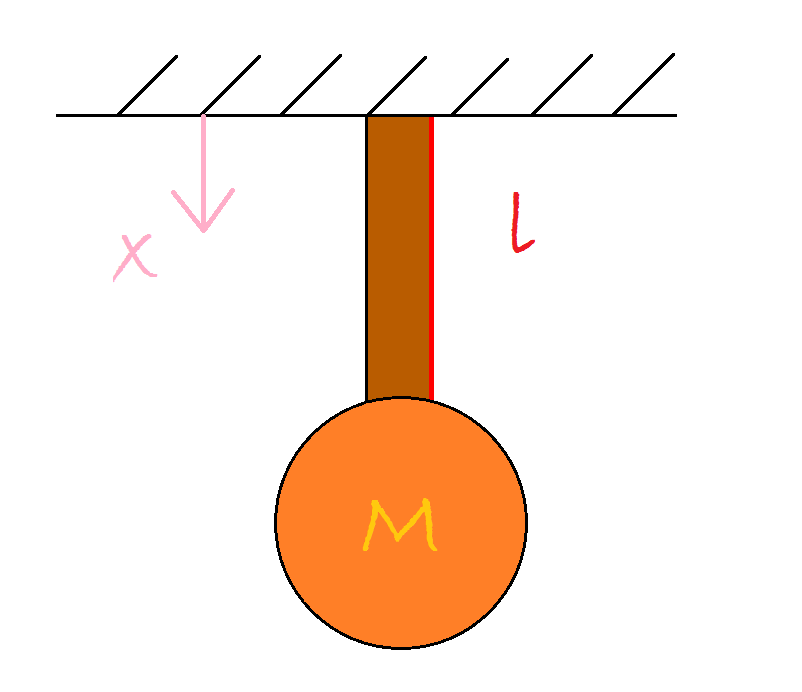
\includegraphics[height=3.5cm]{./pelda.png} %pelda.png
	\centering
	\caption{Felfüggesztett rúd aljára tömeget akasztunk.}
	\label{fig:pelda}
	\end{figure}
\newline
Tegyük meg azt az egyszerűsítő feltevést, miszerint a harántösszehúzódástól eltekintünk:
	\[ \underline{u}(x)=\left(
	\begin{array}{c}
	$$u(x)$$\\
	0\\
	0
	\end{array}\right) \]
Ekkor $\underline{\underline{\sigma}}$-nak is csak $\sigma_{11}$ komponense van, melyet $x$-szerinti deriválással állíthatunk elő:
\[\sigma_{11}=E\frac{\mathrm{d}\underline{u}}{\mathrm{d}x}\]
A mozgásegyenlet baloldalán (minthogy sztatikáról van szó) nulla szerepel:
\[0=\rho\underline{g}+\frac{\mathrm{d}}{\mathrm{d}x}E\frac{\mathrm{d}\underline{u}}{\mathrm{d}x}\]
ahol a második tag $\underline{\nabla}\underline{\underline{\sigma}}$, és
	\[ \underline{g}=\left(
	\begin{array}{c}
	$$g$$\\
	0\\
	0
	\end{array}\right) \]
alakú. Ebből pedig
\[\rho\underline{g}=-E\frac{\mathrm{d}^{2}\underline{u}}{\mathrm{d}x^{2}}\]
mely összefüggés még nem tartalmazza a felakasztott tömeget; kell még peremfeltételt megadnunk, hogy $\underline{u}$-t konkretizálhassuk. (Mint ha $x$ helyére $t$-t írnánk, csak annyit mondhatnánk, hogy állandó a gyorsulás, ám ehhez még szükségünk lenne kezdőfeltételre, melyből kiszámíthatjuk a konkrét mozgást.) A test belsejét leíró differenciálegyenlet ugyanaz igen különböző deformációk esetén is, a konkrét problémát a peremfeltétel adja meg. Ezek esetünkben:
	\begin{itemize}
		\item $u(0)=0$, mivel a rúd teteje nem mozdul el
		\item $Mg=AE\frac{\mathrm{d}u}{\mathrm{d}x}\Big|_{l}$, azaz a belső feszültség és a keresztmetszet szorzata, azaz a belső erő tartja a tömeget ($l$ arra vonatkozik, hogy a rúd végére akasztjuk a tömeget, eddig vizsgáljuk a rúd deformációját)
	\end{itemize}
Ezek alapján $u(x)$-et az alábbi alakban keressük:
\[u(x)=a+bx-\frac{1}{2}\cdot\frac{\rho g}{E}x^{2}\]
Az első peremfeltétel szerint azonban $u(0)=0$, minek alapján $a=0$. Ekkor a fenti Ansatzot a második peremfeltételbe helyettesítve:
\[Mg=AE\bigg(b-\frac{1}{2}\cdot\frac{\rho g}{E}2l\bigg)\]
Melyből átrendezéssel, 2-vel való egyszerűsítéssel, és felhasználva, hogy $Al=V$, s $\rho V=m$
\[Mg+\rho gAl=(M+m)g=AEb\]
amiből
\[b=\frac{Mg}{AE}+\frac{\rho g}{E}l=\frac{g}{AE}(M+m)\]
tehát
\[u(x)=\frac{g}{AE}(M+m)x-\frac{1}{2}\cdot\frac{\rho g}{E}x^{2}\]
azaz \textbf{parabola szerint nyúlik meg}.
\newline
Végül vizsgáljuk meg a határeseteket!
	\begin{itemize}
		\item amikor $\rho=0$, ekkor $u(x)=\frac{g}{AE}(M+m)x$, azaz úgy viselkedik, mint egy egyenletesen megnyúló (elhanyagolható tömegű) rugó /$u(l)=\frac{F}{AE}l$, amiből $F=\frac{AE}{l}\Delta l$, ahol $\frac{AE}{l}=D$/
		\item amikor pedig $M=0$, ez esetben láthatjuk; saját súlya alatt feleannyit nyúlik, mintha egész tömegét súlytalan rugó végére tennénk.
	\end{itemize}

\end{document}
